\documentclass{article}
\usepackage[utf8]{inputenc}
\usepackage{graphicx}
\usepackage{booktabs}
\usepackage[margin=1in]{geometry}
\usepackage{url}
\usepackage[toc,page]{appendix}
\usepackage{lscape}
\usepackage{subcaption}
\usepackage{longtable}
\usepackage[hidelinks]{hyperref}
\usepackage{biblatex} %Imports biblatex package
\usepackage{fancyhdr}
\usepackage{lastpage}
\usepackage{framed}
\usepackage{pgfplots}
\usepackage[T1]{fontenc}
\usepackage{subcaption}
\usepackage{amsmath, amsthm, amssymb, amsfonts}
\newcommand{\textbox}[2][6]{
\begin{framed}
\noindent#2
\end{framed}}

\addbibresource{bibliography.bib} %Import the bibliography file \title{Threat Analysis: a Patient Monitoring System}
\author{Robin Martens}
\date{19/08/2023}

\newcommand{\tabitem}{\textbullet \ }
\newcommand{\https}{\textsc{https}}
\newcommand{\smtp}{\textsc{smtp}}
\newcommand{\threat}[4]{#1 & \textit{#2} & #3 & #4 \\}

\renewcommand{\sectionmark}[1]{\markright{\thesection.\ #1}}

\fancyhead[L]{Robin Martens: r0885874}
\fancyhead[C]{}
\fancyhead[R]{}
\fancyfoot[L]{Report Project I}
\fancyfoot[C]{}
\fancyfoot[R]{\thepage /\pageref{LastPage}}

\renewcommand{\headrulewidth}{0.4pt}
\renewcommand{\footrulewidth}{0.4pt}

\definecolor{s}{HTML}{25282a}
\definecolor{t}{HTML}{003b56}
\definecolor{r}{HTML}{0d514c}
\definecolor{i}{HTML}{0f471f}
\definecolor{d}{HTML}{473300}
\definecolor{e}{HTML}{522000}

\newcounter{assumptioncounter}
\DeclareRobustCommand{\assumption}{%
   \refstepcounter{assumptioncounter}%
   \textit{AS\theassumptioncounter :}~}

\begin{document}
\begin{titlepage}
    \newpage
    \pagenumbering{Roman}
    \thispagestyle{empty}
    \frenchspacing
    \hspace{-0.2cm}
    \hspace{0.2cm}
    \hspace{0.2cm}
    
\includegraphics[height=2.5cm]{images/misc/logoFirW.jpg}
    \hspace{5.8cm}
    
\includegraphics[height=2.5cm]{images/misc/kul_logo.jpg}
    \hspace{\stretch{1}}
    \vfill
    \vspace{0.5cm}
    \centering\Large{\rm\textbf{{Computer Algebra for Cryptography}}}
    \vspace{5cm}
    \begin{center}
        \begin{minipage}[t]{\textwidth}
            \begin{center}
                \Huge{\rm\textbf{Project I}} \\
                \vspace{0.5cm}
                \large{\rm\textsc{{final report}}} \\
                \vspace{1cm}
                {\rm {Robin Martens}} \\
                \vspace{9cm}
                \LARGE{\rm\textsc{academic year 2024-2025}}
                \vfill
            \end{center}
        \end{minipage}
    \end{center}
    \vfill
\end{titlepage}


\pagenumbering{arabic}
\setcounter{page}{1}
\pagestyle{fancy}


\subsection*{Task 1}
\subsubsection*{Task 1.e}

\begin{figure}[htpb]
  \centering
  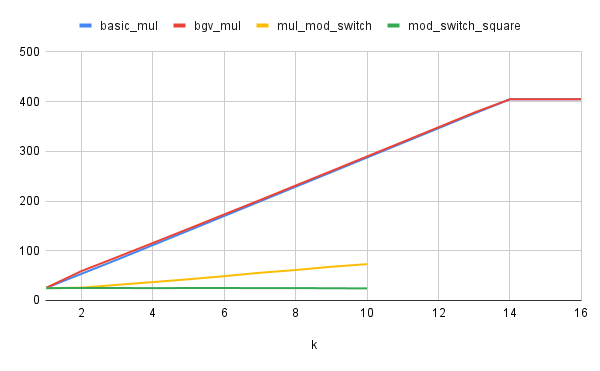
\includegraphics[width=0.8\textwidth]{./chart.png}
  \caption{Plot of the different noise bounds for the cases given in the
  assignment.}
  \label{fig:plot}
\end{figure}

Figure~\ref{fig:plot} shows the noise bound for using just \texttt{BGVBasicMul}
(in blue), for \texttt{BGVMul} (in red), for \texttt{BGVMul}, followed by a
\texttt{BGVModSwitch} (in yellow) and for the repeated squaring (in green). We
here clearly see why the modulus switching is necessary to prevent a build up of
noise in the ciphertext. Note that the $y$-axis displays the logarithm of the
actual noise bound as defined in the assignment.

We see a similar pattern for both \texttt{BGVBasicMul} and \texttt{BGVMul},
which can be explained by the fact that the length of the ciphertext does not
influence the noise bound (as we take the infinity norm of the partial decrypt,
which is already central reduced). The quadratic noise growth is explained by
working out the decryption of the product of two ciphertexts:
\begin{equation}
  \begin{split}
    \mathcal{D}\left( \texttt{ct} \cdot \texttt{ct}'\right) &= \left(
      \mathbf{c}_0 + \mathbf{c}_1
    \cdot \mathbf{s} \right) \cdot (\mathbf{c}_0^\prime + \mathbf{c}_1^\prime
    \cdot \mathbf{s}) \\
                                                            &= (\mathbf{m} + p
                                                            \mathbf{e}) \cdot
                                                            (\mathbf{m}' + p
                                                            \mathbf{e}') \\
                                                            &=
                                                            \mathbf{m}\mathbf{m}'
                                                            +
                                                            \mathbf{m}\mathbf{e}'
                                                            +
                                                            \mathbf{m}'\mathbf{e}
                                                            +
                                                            \mathbf{e}\mathbf{e}'.
  \end{split}
\end{equation} 

For \texttt{BGVMul}, followed by a
\texttt{BGVModSwitch}, we can clearly see that the noise is reduced to
approximately the original level, by using modulus switching.

\noindent We get a faulty decryption from the moment that the error term of the
decryption $p \mathbf{e}^\prime$ becomes larger than $\frac{q}{2}$. For the
standard parameter set, we get:
\begin{equation}
  \log_2\left(\frac{q}{2}\right) \approx 404.69.
\end{equation} 

When the noise bound comes close to this bound, we get errors in the decryption.
From the figure we can derive that we get errors from $k = 14$ and above. A very
rough bound can be derived from the fact that we have $e_0 2^k < \frac{q}{2}
$. With $\log_2(e_0) \approx 22$, we find $k = 18$, which is higher than we
found in the figure, but is explained by the fact that $\mathbf{m}\mathbf{e}' +
\mathbf{m}'\mathbf{e}$ also contribute to the noise term.

For multiplying a bunch of ciphertexts, we have to perform the \texttt{BGVMul}
with modulus switching, as long as it's possible based on the level $\ell$.
Thereafter, the noise will inevitable grow (approximately) quadratically until
we reach the noise bound and have a faulty decryption.

\subsection*{Task 4}

\subsubsection*{Task 4.a}

The intuition is that the error on the equations cannot become too large w.r.t.
the value of the equation itself. If we take the worst case, the maximum value
of a single equation is $(q - 1)n$ (we can take a more liberal bound if we take
into account that $\frac{1}{3}$ of the secret key is supposed to be $0$, or
even more liberal if take into account the cancellation due to the $1$ and $-1$
in the secret key). The maximum value of an error coefficient is $B$, so we get
the bound \begin{equation}
  (q - 1)n > B.
\end{equation} 

\subsubsection*{Task 4.b}

The idea behind the lattice attack is to create a lattice where the shortest
vector of the lattice contains the secret key $\mathbf{s}$. We thus have to
create a target vector $\mathbf{t}$ which lies inside the lattice and is much
shorter than the expected shortest vector (using the Gaussian + Stirling
heuristic) in the lattice.

If we want to create an $(n+3)$-dimensional lattice, we consider the following
matrix (where the rows of the matrix form a basis for the lattice): 
\begin{equation}
  M = \begin{bmatrix} 
    1 & \cdots & 0 & 0 & a_1 & 0 & 0 \\
    0 & 1 & \cdots & 0 & a_2 & 0 & 0 \\
    \vdots & & \ddots & 0  & \vdots & 0 & 0 \\
    0 & & & 1 & a_{n} & 0 & 0 \\
    0 & \cdots & \cdots & 0 & p & 1 &  0 \\
    0 & \cdots & \cdots & 0 & B[1] & 0 & 1 \\
    0 & \cdots & \cdots & 0 & q & 0 & 0 \\
  \end{bmatrix}.
\end{equation} 

\noindent The first $n$ columns are just an identity matrix, while the $(n+1)$th
column corresponds to equation (2) (which is the first row of the circular
matrix for the negacyclic convolution, which corresponds to polynomial
multiplication modulo $x^N + 1$), where we have expressed the mod $q$
explicitly as a factor $kq$ in the equation.

This way, if we multiply $M$ with $\begin{bmatrix} \mathbf{s} & E[1] & -1 & k
\end{bmatrix}$, we get:
\begin{equation}
  \begin{bmatrix} 
    \mathbf{s} & E[1] & -1 & k
  \end{bmatrix}
  \cdot M = 
  \begin{bmatrix} \mathbf{s} & 0 & E[1] & 0 \end{bmatrix}.
\end{equation}

\noindent For the volume we have, as $d = n$ :
\begin{equation}
  \det M = q \det(I_{(n + 2) \times (n + 2)}) = q,
\end{equation} 
from which we can calculate the expected length of the shortest vector $\lambda_1(L)$ : 
\begin{equation}
  \begin{split}
    \lambda_1(L) &\approx \sqrt{\frac{d}{2 \pi e}} \text{vol}(L)^{1 / d} \\
                 &\approx \sqrt{\frac{N+3}{2 \pi e}} q^{\frac{k}{N+3}},
  \end{split}
\end{equation} 
if we take $q$ to be of the form $q^k$. The expected length of $\mathbf{t}$ is
(worst case):
\begin{equation}
  \|\mathbf{t}\| \approx \sqrt{\frac{2}{3}N + B^2},
\end{equation}
as $\mathbf{s}$ is taken uniformly and is ternary, so $\frac{2}{3}$ of the
elements are either $1$ or $-1$. If we combine the above two equations and solve
for $k$, we find:
\begin{equation}
k \ge 4.07.
\end{equation} 

If we wouldn't take out $p$ explicitly from $E[1]$, we could not put $p$ in the
matrix as above and we cannot put $pE[1]$ in the target vector, as it would be
too large (or we would have to take $k$ very large).

\subsection*{Task 4.d}
Experimentally, we find that we find the correct vector for $k \ge 5$, which
corresponds to the bound for $k$ found in the previous subtask.


\subsection*{Task 5}

\subsubsection*{Task 5.a}

For $k = 2$, the decryption equation becomes
\begin{equation}
  \mathbf{r} = \left[\texttt{ct}[0] + \texttt{ct}[1] \mathbf{s}\right]_q \mod p.
\end{equation} 

\noindent As $\mathbf{s}$ is small, it will not be central reduced, nor be
reduced mod $p$ (if $p > 2$), such that if we plug in $\texttt{ct} = [0, 1]$,
we get $\mathbf{r} = \mathbf{s}$.

If $p = 2$, however, the $\text{mod}\ p$, \textit{will} reduce $\mathbf{s}$ (in
this case, as $\mathbf{s}$ is ternary, all the $-1$ will be reduced to $1$.

\subsubsection*{Task 5.c}

As explained above, there will be a decryption error when the noise term of the
partial decryption is greater than $\frac{q}{2}$, as then the noise wraps around
due to the centered reduction. Now, by construction we have $q = 1 \mod p$ and
thus $(q - 1) = 0 \mod p$ and also $\frac{q-1}{2} = 0 \mod p$. Secondly, we note
that

\begin{equation}
  \begin{cases}
    \frac{q-1}{2} < \frac{q}{2} \\
    \frac{q-1}{2} + 1 > \frac{q}{2}
  \end{cases}.
\end{equation} 

\noindent This means that if we create a ciphertext with noise bound
$\frac{q-1}{2}$, it will be a bordeline case. Thirdly, we notice that the noise
term is always a multiple of $p$ and that by adding multiples of $p$ to the
any part of the ciphertext will not change the decryption as long as we don't
surpass the noise bound.

We start with the public key as a valid ciphertext, which is defined as
\begin{equation}
  \mathbf{b} = \mathbf{a} \cdot \mathbf{s} + p \mathbf{e},
\end{equation}
where the coefficients of $\mathbf{e}$ are in the interval $[-B, B]$, with $B$
small. The fact that $B$ is small can be exploited as follows. Suppose that the
$i$th coefficient of $\mathbf{e}$ is $e_i \in [-B, B]$. Now we add
$\frac{q-1}{2}$ to $e_i$, such that we either have an overshoot or undershoot of
the noise bound (depending on the fact of the original $e_i$ was positive or
negative). Note that in the special case that $e_i = 0$, we are already at the
noise bound. In general, we then loop twice over the interval $[1, B]$. In the
first round, we subtract $p$ from $e_i$ (to test for overshoot) and in the
second round, we add $p$ to $e_i$ (to test for undershoot). Somewhere in this
looping, we reach the bound $\frac{q-1}{2}$, which indicates that we found
$e_i$.

The final things which we have to do is finding a way to check if we reached the
bound $\frac{q-1}{2}$, as we do not have access to the
\texttt{BGVPartialDecrypt} method. If some $e_i = \frac{q-1}{2}$, the decryption
will still be correct, but if we add $1$ to $e_i$, we get (taking into account
the centered reduction):
\begin{equation}
  \frac{q-1}{2} + 1 - q = \frac{1-q}{2} = - \frac{q-1}{2},
\end{equation} 
which is \textit{still} a multiple of $p$, such that it disappears modulo $p$.
This indicates that we still get the original message that we encrypted, which
is a decryption failure, as we should get $\mathbf{m} + 1$, following the
decryption equation. It suffices thus to check that \texttt{BGVDecrypt(ct, sk)
} \texttt{eq} \ \texttt{BGVDecrypt(<[ct[1][1]+1, ct[1][2]], ct[2]>, sk)}. \\

This can also be generalized to work for all coefficients at the same time.
Then, the followings steps should be adapted:
\begin{itemize}
  \item Instead of adding $\frac{q-1}{2}$ in the first step, we add the
    polynomial of degree $N-1$ with all coefficients equal to $\frac{q-1}{2}$
    (i.e. $\sum_{n=0}^{N-1} \left( \frac{q-1}{2} \right) x^i$).
  \item In the iterations, we do a similar change: instead of adding $p$, we add
    the polynomial of degree $N-1$ with all coefficients equal to $p$.
  \item To check which coefficients already reached the threshold, we add a
    polynomial of degree $N-1$ with all coefficients 1 and decrypt. We then
    check which coefficients are equal (using the principle described above) to
    the decryption of the ciphertext before we added the polynomial.
\end{itemize}

The methods where we find all coefficients at once is \textit{much} more
efficient then the algorithm where all coefficients are found one by one
(experimentally up to a factor 40 less).
 
\subsection*{Task 6}

\subsubsection*{Task 6.c}
Yes, if we want to multiply polynomials over the ring $\mathbb{Z}_q[x] \setminus
\left( x^N - 1 \right) $, we have to use the so-called positive wrapped
convolution or cyclic convolution and for working over the ring $\mathbb{Z}_q[x]
\setminus \left( x^N + 1 \right) $, we have to do use the so-called negative
wrapped convolution (or negacyclic convolution). The main point is that by
evaluating the \textsc{ntt} in the roots of $(x^N - 1)$, we're working in the
above mentioned ring. We can use the same principle to work over the ring module
$(x^N + 1)$, namely by evaluating the \textsc{ntt} in the roots $(x^N + 1)$
instead of the roots of $(x^N - 1)$. We call these roots $\psi$, the $2n$-th
root of unity such that $\psi^2 = \omega$ in $\mathbb{Z}_q$, as $x^{2n} - 1 = (x^n -
1)(x^n + 1)$. We can then evaluate the \textsc{ntt} in the odd powers of $\psi$,
which gives \cite{ntt-2023, satriawan-2023}:
\begin{equation}
  \begin{split}
    \textsc{ntt}_\psi (a)_j &= \sum_{i= 0}^{n - 1} a_i \psi_{2n}^{i (2j +1)} \\
                            &= \sum_{i = 0}^{n-1} a_i \omega_n^{ij} \psi_{2n}^i
                            \\
                            &= \textsc{ntt}_\omega\left( \left[ \psi_{2n} a_0,
                            \dots, \psi_{2n}^{n-1} a_{n-1} \right]  \right) 
  \end{split}
\end{equation} 

\subsubsection*{Task 6.d}

Yes, we could use the \textsc{ntt} and the \textsc{intt} to do the encoding. The
main idea of encoding is to perform multiplication and addition in $R_p$, which
is then a point-wise multiplication in $\mathbb{F}_p$. As we want to have
pointwise multiplication over a sequence in $\mathbb{F}_p$, which corresponds to
multiplication in $R_p$, we take the inverse \textsc{ntt} for encoding and the
\textsc{ntt} for decoding.

\clearpage

\printbibliography

\end{document}
